\documentclass[twocolumn,floatfix]{article}
\usepackage[utf8x]{inputenc}
\usepackage[pdftex]{graphicx}
\usepackage{mathpazo} 
\usepackage{amsmath}
\usepackage{amsfonts}
\usepackage{amssymb}
\usepackage{braket}
\usepackage{dsfont}
\usepackage[pdftex]{hyperref}   
\usepackage{siunitx}
\usepackage{bbm, dsfont}
\usepackage[font=small]{caption}
\usepackage[margin=1in]{geometry}
\usepackage{float}
\usepackage{tikz}
\usetikzlibrary{arrows,shapes,trees}

\graphicspath{{images/},{figures/}}

\title{Systems with a strong interaction to an enviroment}
\author{Eduardo Villase\~nor}
\date{\today}

\begin{document}
\maketitle



\section{Introduction}

We are interested in studying a central spin 1/2 system that has a strong interaction to an 
environment. To accomplish this, we simulate the environment $E$ using a kicked spinchain and have
our central system $C$ having some strong interaction with some parts of this spinchain.

As a first exploration, two similar models were used as fig. \ref{models} shows. Having in the
first model the central system interaction with only one of the parts of the chain, in contrast
with the second one in which the central system interacts with three parts of the chain.


\begin{figure}[H]
\begin{center}
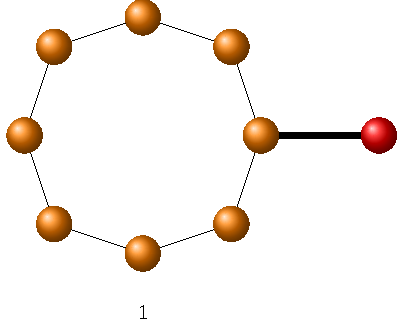
\includegraphics[width=.49\columnwidth]{model1} \hfill
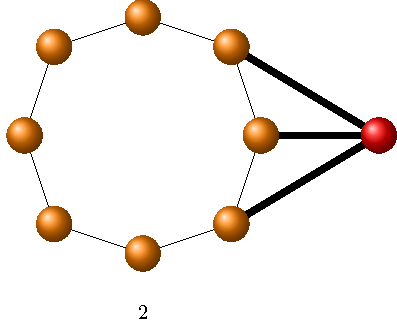
\includegraphics[width=.49\columnwidth]{model2} 
\end{center}
\caption{Visual representation of the two models used. The orange dots
represent the environment $E$ and the red one the central system $C$.}
\label{models}
\end{figure}

To describe the model we introduce the Hamiltonians for $H_{CE}$ the interaction between $C$ and $E$, and $H_{E}$ for the internal interaction 
between the particles in the environment.
\begin{equation}
H_{CE}=J_c\sum_{i,j} \sigma_i^z \sigma_j^z; \quad H_{E}=  \sum_{k \in E} J_{k} \sigma_{k}^z \sigma_{k+1}^z.
\end{equation}
The Ising interaction between each of the the spins on the chain is randomized,
such that $J_k \in [J_s-\Delta J_s,J_s+\Delta J_s]$.
Thus the Ising Hamiltonian that describes the complete model
\begin{equation}
H_{I}=H_{CE} + H_{E}.
\end{equation}

Additionally, the magnetic field Hamiltonian described as usual for the entire model.
\begin{equation}
H_{II}=\sum_{i} \vec{\sigma_i} \cdot \vec{b},
\end{equation}
where we can always chose a reference frame were the field is only $b_x$ and $b_z$.

We see that the system is characterized by the set of parameters
$[J_c,J_s,\Delta J_s,bx,by]$.  Also we must mention that over this full work
the initial state of the system $\Ket{\psi} = \Ket{\psi_{\rm rand}^{E}}  \otimes \Ket{\psi_{\rm rand}^{C}} $ was
always used.

\section{Finding the correct parameters}
We are interested in finding the correct parameters in which the system has an chaotic behaviour.
To accomplish this we analyse the systems spectral density and the nearest neighbour distribution.
For both models with the parameters $[1.4,1.4,0.2,1.4,1.4]$ we found such behaviour as fig \ref{ps_model1}
and fig. \ref{ps_model2} show for models 1 and 2 respectively. 
\begin{figure}[H]
\begin{center}
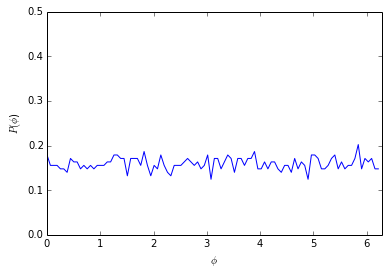
\includegraphics[width=.49\columnwidth]{spectra_model1} \hfill
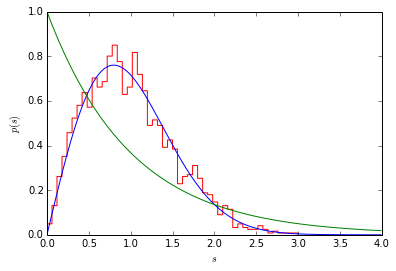
\includegraphics[width=.49\columnwidth]{ps_model1} 
\end{center}
\caption{(left)Spectral density and (right)the nearest neighbour distribution for model 1.}
\label{ps_model1}
\end{figure}
\begin{figure}[H]
\begin{center}
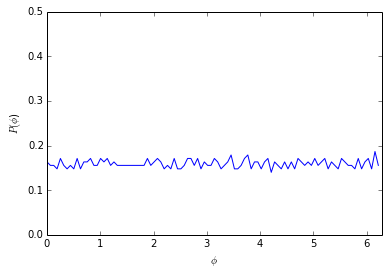
\includegraphics[width=.49\columnwidth]{spectra_model2} \hfill
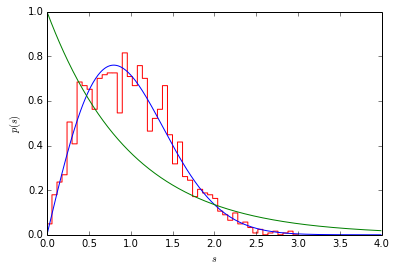
\includegraphics[width=.49\columnwidth]{ps_model2} 
\end{center}
\caption{(left)Spectral density and (right)the nearest neighbour distribution for model 2.}
\label{ps_model2}
\end{figure}

It's important to note that different values of
$J_c$ were used, fixing the other parameters, and a very similar behaviour was found.
And so the set of parameters to be used is $P=[J_c,1.4,0.2,1.4,1.4]$.




\section{Purity decay of $C$}
First we are interested in knowing how much the randomness of the 
system (in the parameters $J_k$) affects the Purity of $C$.
We calculate the Purity over times as $\gamma(t)= {\rm Tr}(\rho (t)^2)$, where $\rho(t)$ corresponds to
the reduced density matrix of $\Ket{\psi(t)}$ over $C$.
The results in fig. \ref{randomness} show how for small values of $J_c$ there is a considerable variation 
for different {\it runs} of the system, however for larger values of $J_c$ there is no considerable 
variation.
\begin{figure}[H]
\begin{center}
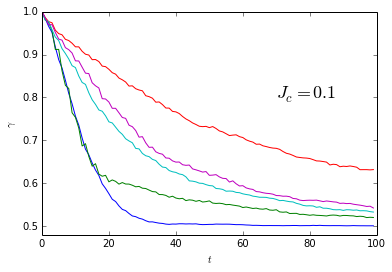
\includegraphics[width=.49\columnwidth]{aleatoriedad} \hfill
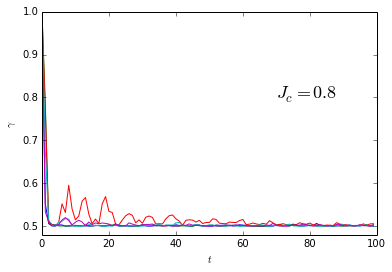
\includegraphics[width=.49\columnwidth]{aleatoriedad2} 
\end{center}
\caption{Different {\it runs} using model 1, were different random variables $J_k$ were created using parameters $P$ and fixed $dim(E)=10$
The left panel corresponds with $J_c=0.1$, and the right panel to $J_c=0.8$.  }
\label{randomness}
\end{figure}


\subsection{Varying the size of $E$}
Now we explore the purity when we vary the size of $E$. The results for purity decay in
each of the models are shown of fig. \ref{varE}.
\begin{figure}[H]
\begin{center}
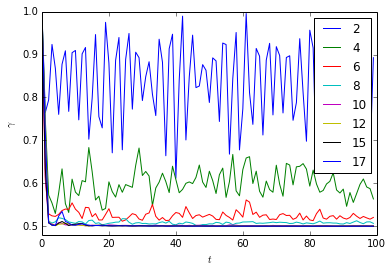
\includegraphics[width=.49\columnwidth]{qubits_model1} \hfill
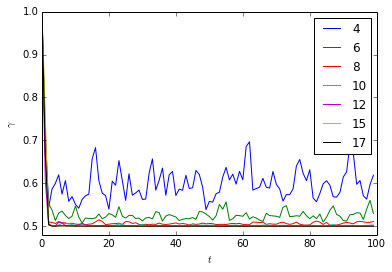
\includegraphics[width=.49\columnwidth]{qubits_model2} 
\end{center}
\caption{Purity decay fixing the value $J_c=0.8$ and using $P$ for the other parameters.
The legend shows the total dimension of the system, that is $dim(E)+1$.
The left panel
shows for model 1 and the right one shows model 2.}
\label{varE}
\end{figure}

\subsection{Varying the parameter $J_c$}
To complete the exploration for these two models, we now fix all the variables and
vary the parameter $J_c$. Our interests now is in finding the behaviour of the purity $\gamma$
for long times. To do so we define the average over two points in times as
\begin{equation}
<\gamma>_{T_1}^{T_2} = \frac{1}{T_2-T_1+1} \sum_{t=T_1}^{T_2} \gamma(t).
\end{equation}

Fig. \ref{varj} show the calculations for $<\gamma>_{80}^{100}$ obtained for both models.
\begin{figure}[H]
\begin{center}
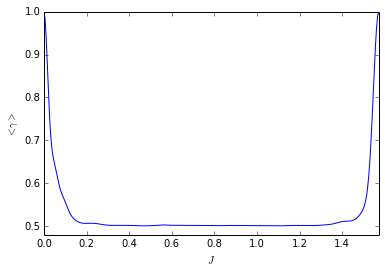
\includegraphics[width=.49\columnwidth]{varj_model1} \hfill
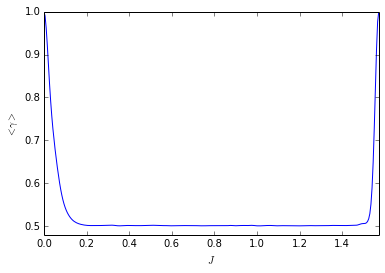
\includegraphics[width=.49\columnwidth]{varj_model2} 
\end{center}
\caption{Values $<\gamma>_{80}^{100}$ varying $J_c$, with parameters $P$ and 
a total of 10 qubits. For both models, 1 and 2, left and right respectively.}
\label{varj}
\end{figure}

We see how for both models the behaviour of $\gamma$, in long times, basically goes to its lowest
value possible with the exception where the system becomes trivial near $J_c=0$ and $J_c=\frac{\pi}{2}$ being 
$J_c$ $\frac{\pi}{2}$-periodic.









\end{document}